\documentclass[tikz,border=6pt]{standalone}
\usepackage[T1]{fontenc}
\usepackage[utf8]{inputenc}
\usepackage{pgfplots}
\usepgfplotslibrary{groupplots}
\usetikzlibrary{calc}
\pgfplotsset{compat=1.18}
\begin{document}
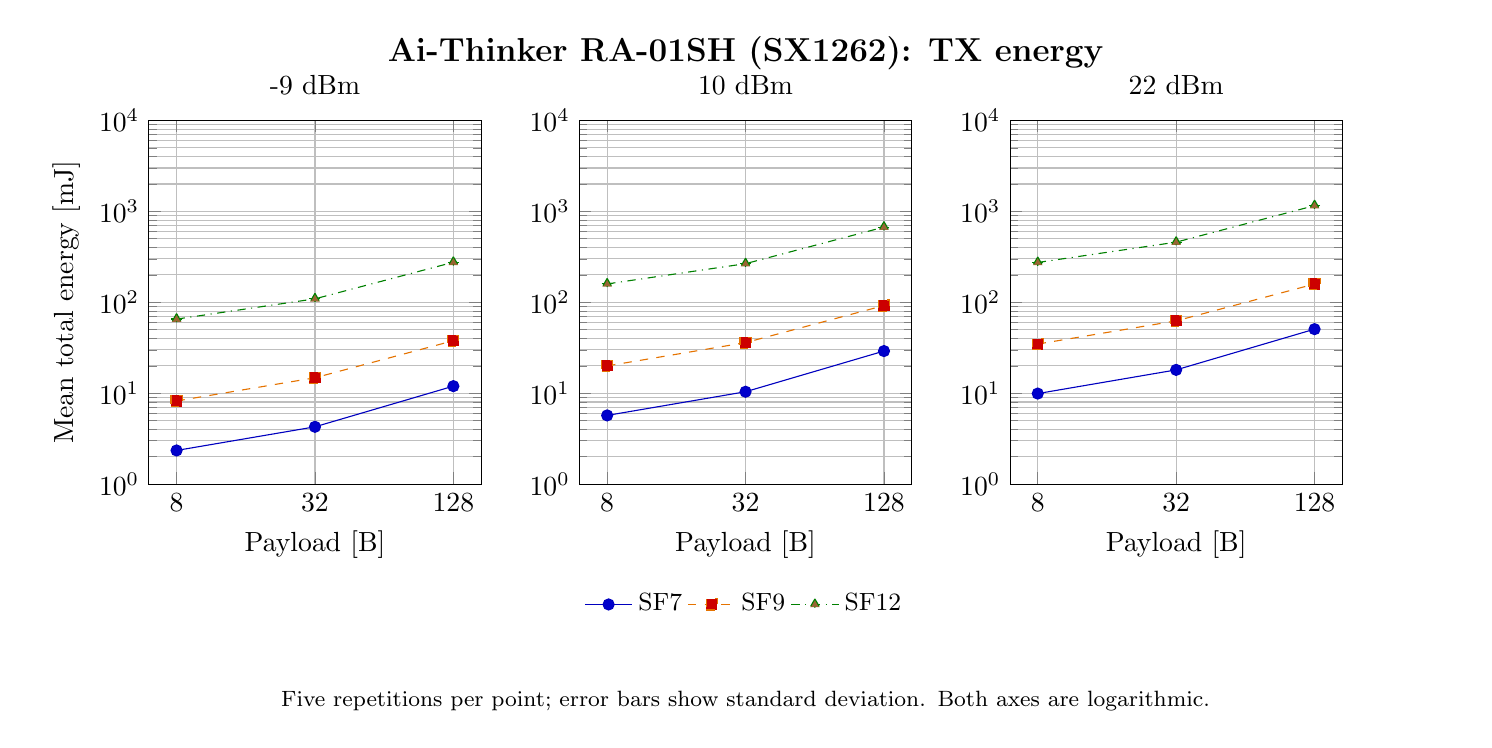
\begin{tikzpicture}
\begin{groupplot}[/pgf/number format/use comma, group style={group size=3 by 1, horizontal sep=1.25cm},
  width=5.8cm,height=6.2cm,xmode=log,log basis x=2,ymode=log,log basis y=10,ymin=1,ymax=10000,
  xtick={8,32,128},xticklabels={8,32,128},grid=both,xlabel={Payload [B]},
  legend style={draw=none,fill=none,font=\small,at={(0.5,-0.27)},anchor=north,legend columns=-1}]
% TX energy
\nextgroupplot[title={-9 dBm},ylabel={Mean total energy [mJ]}]
\addplot+[blue!75!black,solid,mark=*,error bars/.cd,y dir=both,y explicit] coordinates {(8,2.34317612) +- (0,0.00333362355) (32,4.26297598) +- (0,0.00401986597) (128,11.9432684) +- (0,0.0148400772)};
\addplot+[orange!90!black,dashed,mark=square*,error bars/.cd,y dir=both,y explicit] coordinates {(8,8.20249759) +- (0,0.00942113332) (32,14.7659451) +- (0,0.0261478481) (128,37.7508038) +- (0,0.0409711462)};
\addplot+[green!50!black,dashdotted,mark=triangle*,error bars/.cd,y dir=both,y explicit] coordinates {(8,65.2736743) +- (0,0.0770516986) (32,109.017169) +- (0,0.0890415612) (128,275.320753) +- (0,0.114322523)};
\nextgroupplot[title={10 dBm}]
\addplot+[blue!75!black,solid,mark=*,error bars/.cd,y dir=both,y explicit] coordinates {(8,5.69146891) +- (0,0.00561827486) (32,10.3655693) +- (0,0.00843610807) (128,29.0528797) +- (0,0.0140958257)};
\addlegendentry{SF7}
\addplot+[orange!90!black,dashed,mark=square*,error bars/.cd,y dir=both,y explicit] coordinates {(8,19.947014) +- (0,0.0116622302) (32,35.9698816) +- (0,0.0277375841) (128,91.9527946) +- (0,0.0314553339)};
\addlegendentry{SF9}
\addplot+[green!50!black,dashdotted,mark=triangle*,error bars/.cd,y dir=both,y explicit] coordinates {(8,159.055538) +- (0,0.0348288016) (32,265.676944) +- (0,0.0590021885) (128,670.792736) +- (0,0.0880124625)};
\addlegendentry{SF12}
\nextgroupplot[title={22 dBm}]
\addplot+[blue!75!black,solid,mark=*,error bars/.cd,y dir=both,y explicit] coordinates {(8,9.89700879) +- (0,0.0426765246) (32,18.0320918) +- (0,0.104832839) (128,50.5950462) +- (0,0.243137607)};
\addplot+[orange!90!black,dashed,mark=square*,error bars/.cd,y dir=both,y explicit] coordinates {(8,34.6842652) +- (0,0.178394176) (32,62.3938419) +- (0,0.384677416) (128,158.66023) +- (0,0.853439053)};
\addplot+[green!50!black,dashdotted,mark=triangle*,error bars/.cd,y dir=both,y explicit] coordinates {(8,273.830385) +- (0,0.390850427) (32,458.142183) +- (0,1.07677951) (128,1156.00195) +- (0,1.48480862)};
\end{groupplot}
\node[font=\bfseries\large] at ($(group c2r1.north)+(0,0.85cm)$) {Ai-Thinker RA-01SH (SX1262): TX energy};
\node[font=\footnotesize,align=center,text width=18cm] at ($(group c2r1.south)+(0,-2.75cm)$) {Five repetitions per point; error bars show standard deviation. Both axes are logarithmic.};
\end{tikzpicture}
\end{document}
